\achapter{25}{Projections onto Subspaces and the Gram-Schmidt Process in $\R^n$} \label{chap:gram_schmidt}

\vspace*{-17 pt}
\framebox{
\parbox{\dimexpr\linewidth-3\fboxsep-3\fboxrule}
{\begin{fqs}
\item What is a projection of a vector onto a subspace and why are such projections important?
\item What is a projection of a vector orthogonal to a subspace and why are such orthogonal projections important?
\item What is the Gram-Schmidt process and why is it useful? 
\item What is the QR-factorization of a matrix and why is it useful? 
\end{fqs}}}% \hspace*{3 pt}}

\vspace*{13 pt}

\csection{Application: MIMO Systems}      
\label{sec:mimo}

MIMO (Multiple Input Multiple Output) systems are widely used to increase data transmission rates and improve the quality of wireless communication systems.  MIMO is one of several forms of smart antenna technology, and it makes use of multiple antennas at the transmitter to send signals and multiple antennas at the receiver to accept the signals. MIMO systems transmit the same data on multiple streams, which introduces redundancy into the system. MIMO systems can utilize bounced and reflected signals to actually improve signal strength. This is very useful in urban environments in the presence of large buildings and the absence of direct line-of-sight transmission. MIMO systems can transmit several information streams in parallel (known as spatial multiplexing), allowing for increased data transformation rates. The presence of multiple receiver antennas allows for greater reliability in the system. 

\begin{figure}[ht]
\begin{center}
\resizebox{!}{1.5in}{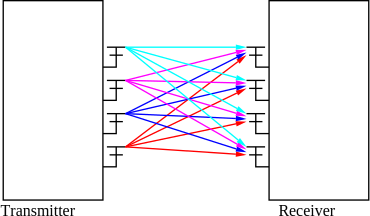
\includegraphics{MIMO.eps}}
\caption{A MIMO system.}
\label{F:MIMO}
\end{center}
\end{figure}
In a MIMO system, every transmitter antenna sends a signal to every receiver antenna as illustrated in Figure \ref{F:MIMO}. In each of these transmissions the signal can be disturbed in some way. Two types of disturbances are \emph{fading} and \emph{noise}. Fading is due to time variations in the received signal, which can occur because of atmospheric conditions or obstacles over the path which are varying with respect to time. In a MIMO system we have \emph{multipath fading} for the different paths the signal takes from different antennas to receivers, which causes fluctuations in amplitude, phase and angle of arrival of the received signal. Noise is an unwanted signal which interferes with actual signal. Both fading and noise result in a received signal that is different than the transmitted signal. The problem is how to recover the original signal from the transmitted signal. The QR decomposition is used in this process. To improve the efficiency of MIMO systems, different methods are introduced to determine a QR decomposition. We will discuss MIMO systems in more detail later in this section, and how Householder transformations can be used to find QR decompositions. 

\csection{Introduction}
\label{sec:gram_schmidt_intro}

In many situations (least squares approximations, for example) want to find a vector $\vw$ in a subspace $W$ of $\R^n$ that is the ``best" approximation to a vector $\vv$ not in the subspace. A natural measure of ``best" is to find a vector $\vw$ in $W$, if one exists, such that the distance from $\vw$ to $\vu$ is a minimum. This means we want to find $\vw$ so that the quantity
\[||\vw - \vu ||\]
is as small as possible over all vectors $\vw$ in $W$. To do this, we will need to find a suitable projection of the vector $\vv$ onto the subspace $W$. We have already done this in the case that $W = \Span\{\vw_1\}$  is the span of a single vector -- we can project the vector $\vv$ in the direction of $\vw_1$. Our goal is to generalize this to project a vector $\vv$ onto an entire subspace in a useful way. 

\begin{pa} \label{pa:6_e_1} Let $\CB = \{\vw_1, \vw_2\}$ be a basis for a subspace $W$ of $\R^3$,  where $\vw_1 = [1 \ 0 \ 0]^{\tr}$ and $\vw_2 = [0 \ 1 \ 0]^{\tr}$. Note that $\CB$ is an orthonormal basis for $W$. Let $\vv = [1 \ 2 \ 1]^{\tr}$. Note that $W$ is the $xy$-plane and that $\vv$ is not in $W$ as illustrated in Figure \ref{F:6_d_o_proj}.
	\be
	\item Find the projection $\vu_1$ of $\vv$ onto $W_1 = \Span\{\vw_1\}$. (Hint: See Equation (\ref{eq:6_a_projection}).) 
		
	\item Find the projection $\vu_2$ of $\vv$ onto $W_2 = \Span\{\vw_2\}$.

	\item Calculate the distance between $\vv$ and $\vu_1$ and $\vv$ and $\vu_2$. Which of $\vu_1$ and $\vu_2$ is closer to $\vv$?
			
	\item Show that the vector $\frac{3}{4} [1 \ 2 \ 0]^{\tr}$ is in $W$ and find the distance between $\vv$ and $\frac{3}{4} [1 \ 2 \ 0]^{\tr}$.


\item Part (4) shows that neither vector $\vu_1 = \proj_{\vw_1} \vv$ nor $\vu_2 = \proj_{\vw_2} \vv$ is the vector in $W$ that is closest to $\vv$. We should probably expect this neither projection uses the fact that the other vector might contribute to the closest vector. Let us instead consider the sum $\vu_3 = \vu_1+\vu_2$. Calculate the components of this vector $\vu_3$ and determine the distance between $\vu_3$ and $\vv$. Which of the three vectors $\vu_1$, $\vu_2$, and $\vu_3$ in $W$ is closest to $\vv$?  

	
\item A picture of $\vw_1$, $\vw_2$, $W$, and $\vv$ is shown in Figure \ref{F:6_d_o_proj}. Draw in $\vu_1$, $\vu_2$, and $\vu_3$. Draw a picture of the vector $\vw$ in $W$ that appears to be closest to $\vv$. Does this vector seem to have any relationship to $\vu_1$, $\vu_2$, or $\vu_3$? If yes, what relationship do you see?
\begin{figure}[h]
\begin{center}
\resizebox{!}{2.5in}{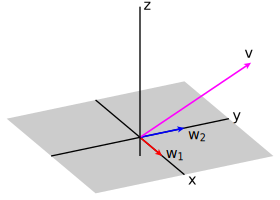
\includegraphics{6_d_O_proj}}
\end{center}
\caption{The space $W$ and vectors $\vw_1$, $\vw_2$, and $\vv$.}
\label{F:6_d_o_proj}
\end{figure}


	\ee
\end{pa}


\csection{Projections onto Subspaces and Orthogonal Projections }
\label{sec:proj_subsp_orth}

Preview Activity \ref{pa:6_e_1} gives an indication of how we can project a vector $\vv$ in $\R^n$ onto a subspace $W$ of $\R^n$. If we have an orthogonal basis for $W$, we can just add the projections of $\vv$ onto each basis vector. The resulting vector is called the projection of $\vv$ onto the subspace $W$. As we did with projections onto vectors, we can also define the projection of $\vv$ orthogonal to $W$. Note that to make this all work out properly, we will see that we need an orthogonal basis for $W$. 

\begin{definition} Let $W$ be a subspace of $\R^n$ and let $\{\vw_1, \vw_2, \ldots, \vw_m\}$ be an orthogonal basis for $W$. The \textbf{projection of the vector $\vv$ in $V$ onto $W$}\index{projection onto a subspace!in $\R^n$} is the vector
\[\proj_W \vv = \frac{\vv \cdot \vw_1}{\vw_1 \cdot \vw_1} \vw_1 + \frac{\vv \cdot \vw_2}{\vw_2 \cdot \vw_2}  \vw_2 + \cdots + \frac{\vv \cdot \vw_m}{\vw_m \cdot \vw_m}  \vw_m.\]
The \textbf{projection of $\vv$ orthogonal to $W$}\index{projection orthogonal to a subspace} is the vector
\[\proj_{\perp W} \vv = \vv - \proj_W \vv.\]
\end{definition}

The notation $\proj_{\perp W} \vv$ indicates that we expect this vector to be orthogonal to every vector in $W$. We address this in the following activity. 

\begin{activity} \label{act:6_e_orth_projection} Let $W = \Span \{\vw_1, \vw_2\}$ in $\R^3$, with $\vw_1=[1 \ 0 \ 0]^{\tr}$ and $\vw_2= [0 \ 1 \ 0]^{\tr}$,  and  $\vv = [1 \ 2 \ 1]^{\tr}$ as in Preview Activity \ref{pa:6_e_1}. Recall that $\proj_W \vv =  [1 \ 2 \ 0]^{\tr}$. Find the projection of $\vv$ orthogonal to $W$ and show directly that $\proj_{\perp W} \vv$ is orthogonal to the basis vectors for $W$ (and hence to every vector in $W$).

\end{activity}

Activity \ref{act:6_e_orth_projection} indicates that the vector $\proj_{\perp W} \vv$ is in fact orthogonal to every vector in $W$. To see that this is true in general, let $\CB = \{\vw_1, \vw_2, \ldots, \vw_m\}$ be an orthogonal basis for a subspace $W$ of $\R^n$ and let $\vv$ be a vector in $\R^n$. Let 
\[\vw =  \proj_W \vv = \frac{\vv \cdot \vw_1}{\vw_1 \cdot \vw_1} \vw_1 + \frac{\vv \cdot \vw_2}{\vw_2 \cdot \vw_2}  \vw_2 + \cdots + \frac{\vv \cdot \vw_m}{\vw_m \cdot \vw_m}  \vw_m.\]
Then $\vv - \vw$ is the projection of $\vv$ orthogonal to $W$. We will show that $\vv - \vw$ is orthogonal to every basis vector for $W$. Since $\CB$ is an orthogonal basis for $W$, we know that $\vw_i \cdot \vw_j = 0$ for $i \neq j$. So if $k$ is between 1 and $m$ then
\begin{align*}
\vw_k \cdot (\vv - \vw) &= (\vw_k \cdot \vv) - (\vw_k \cdot \vw) \\
	&= (\vw_k \cdot \vv) - \left[\vw_k \cdot \left(\ds \frac{\vv \cdot \vw_1}{\vw_1 \cdot \vw_1} \vw_1 + \frac{\vv \cdot \vw_2}{\vw_2 \cdot \vw_2}  \vw_2 + \cdots + \frac{\vv \cdot \vw_m}{\vw_m \cdot \vw_m}  \vw_m \right)\right] \\
	&= (\vw_k \cdot \vv) - \left(\frac{\vv \cdot \vw_k}{\vw_k \cdot \vw_k}\right) (\vw_k \cdot \vw_k) \\
	&= (\vw_k \cdot \vv) - (\vv \cdot \vw_k) \\
	&= 0.
\end{align*}
So the vector $\vv - \vw$ is orthogonal to every basis vector for $W$, and therefore to every vector in $W$ (Theorem \ref{thm:6_a_dot_pd_orth_complement_basis}).  Because $\CB$ is a basis for $W$, if $\vx$ is in $W$, then 
\[\vx = c_1 \vw_1 + c_2 \vw_2 + \cdots + c_m \vw_m\]
for some scalars $c_1$, $c_2$, $\ldots$, $c_m$. So 
\[(\vv - \vw) \cdot \vx = \sum_{k=1}^m c_k (\vv - \vw) \cdot \vw_k = 0,\]
and so $\vv - \vw$ is orthogonal to every vector in $W$. 

\csection{Best Approximations}
\label{sec:best_approx}

We have seen that $\proj_{\perp W} \vv$ is orthogonal to every vector in $W$, which suggests that $\proj_W \vv$ is in fact the vector in $W$ that is closest to $\vv$. We now verify this fact and conclude that $\proj_W \vv$ is the vector in $W$ closest to $\vv$ and therefore the best approximation of $\vv$ by a vector in $W$.

\begin{theorem} Let $\B = \{\vw_1, \vw_2, \ldots, \vw_m\}$ be an orthogonal basis for a subspace $W$ of $\R^n$ and let $\vv$ be a vector in $\R^n$. Then
\[||\vv - \emph{proj}_W \vv || < || \vv - \vx ||\]
for every vector $\vx$ different from $\emph{proj}_W \vv$ in $W$.
\end{theorem}

\begin{proof} Let $\B = \{\vw_1, \vw_2, \ldots, \vw_m\}$ be an orthogonal basis for a subspace $W$ of $\R^n$ and let $\vv$ be a vector in $\R^n$. Let $\vx$ be a vector in $W$. The vector $\proj_W \vv - \vx$ is in $W$, so is orthogonal to $\proj_{\perp W} \vv = \vv - \proj_W \vv$. Thus, the dotted triangle whose vertices are the tips of the vectors $\vv$, $\vx$, and $\proj_W \vv$ in Figure \ref{F:best_approx} is a right triangle.
\begin{figure}[h]
\begin{center}
\resizebox{!}{2.0in}{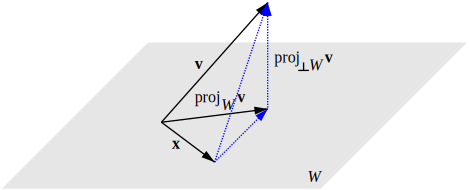
\includegraphics{6_d_best_approx}}
\caption{The best approximation to $\vv$ in $W$}
\label{F:best_approx}
\end{center}
\end{figure}
The Pythagorean theorem then shows that
\[|| \vv - \vx ||^2 = || \proj_{\perp W} \vv ||^2 + || \proj_W \vv - \vx ||^2.\]
Now $\vx \neq \proj_W \vv$, so $|| \proj_W \vv - \vx ||^2 > 0$. This implies
\[|| \vv - \vx ||^2 > || \proj_{\perp W} \vv ||^2\]
and it follows that
\[|| \vv - \vx || > || \proj_{\perp W} \vv ||.\]
\end{proof}
This theorem shows that the distance from $\proj_W \vv$ to $\vv$ is less than the distance from any other vector in $W$ to $\vv$. So $\proj_W \vv$ is the best approximation to $\vv$ of all the vectors in $W$.

If $\vv = [v_1 \ v_2 \ v_3 \ \ldots \ v_m]^{\tr}$ and $\proj_W \vv =  [w_1 \ w_2 \ w_3 \ \ldots \ w_m]^{\tr}$, then the square of the error in approximating $\vv$ by $\proj_W \vv$ is given by
\[|| \vv - \proj_W \vv ||^2 = \sum_{i=1}^m (v_i - w_i)^2.\]
So $\proj_W \vv$ minimizes this sum of squares over all vectors in $W$. As a result, we call $\proj_W \vv$ the \emph{least squares approximation} to $\vv$.

\begin{activity} Let $\CB = \left\{\left[ \begin{array}{r} 1 \\ 0 \\ -1 \\ 0 \end{array} \right], \left[ \begin{array}{r} 0 \\ 1 \\ 0 \\ -1 \end{array} \right], \left[ \begin{array}{r} -1 \\ 1 \\ -1 \\ 1 \end{array} \right]\right\}$ and let $W = \Span(\CB)$ in $\R^4$. Find the best approximation in $W$ to the vector $\vv = \left[ \begin{array}{r} 2 \\ 3 \\ 1 \\ -1 \end{array} \right]$ in $W$.
\end{activity}


\csection{The Gram-Schmidt Process}
\label{sec:gram_schmidt_process}
We have seen that orthogonal bases make computations very convenient. However, until now we had no convenient way to construct orthogonal bases. The problem we address in this section is how to create an orthogonal basis from any basis.  

\begin{pa} \label{pa:6_d_2_no_inner_product}  Let $W = \Span \{\vv_1, \vv_2, \vv_3\}$ in $\R^4$, where $\vv_1 = [1 \ 1 \ 1 \ 1]^{\tr}$, $\vv_2 = [-1 \ 4 \ 4 \ -1]^{\tr}$, and $\vv_3 = [2 \ -1 \ 1 \ 0]^{\tr}$. Our goal in this preview activity is to begin to understand how we can find an orthogonal set $\CB = \{\vw_1, \vw_2, \vw_3\}$ in $\R^4$ so that $\Span \ \CB = W$. To begin, we could start by letting $\vw_1 = \vv_1$. 
	\be
	\item Now we want to find a vector in $W$ that is orthogonal to $\vw_1$. Let $W_1 = \Span\{\vw_1\}$. Explain why $\vw_2 = \proj_{\perp W_1} \vv_2$ is in $W$ and is orthogonal to $\vw_1$. Then calculate the vector $\vw_2$.  


	\item Next we need to find a third vector $\vw_3$ that is in $W$ and is orthogonal to both $\vw_1$ and $\vw_2$. Let $W_2 = \Span \{\vw_1, \vw_2\}$. Explain why $\vw_3 = \proj_{\perp W_2} \vv_3$ is in $W$ and is orthogonal to both $\vw_1$ and $\vw_2$. Then calculate the vector $\vw_3$.  

	\item Explain why the set $\{\vw_1, \vw_2, \vw_3\}$ is an orthogonal basis for $W$. 


	\ee
	
\end{pa}

Preview Activity \ref{pa:6_d_2_no_inner_product} shows the first steps of the Gram-Schmidt process to construct an orthogonal basis from any basis of a subspace in $\R^n$. To understand why the process works in general, let $\{\vv_1, \vv_2, \ldots, \vv_m\}$ be a basis for a subspace $W$ of $\R^n$. Let $\vw_1 = \vv_1$ and let $W_1 = \Span\{\vw_1\}$. Since $\vw_1 = \vv_1$ we have that $W_1 = \Span\{\vw_1\} = \Span\{\vv_1\}$. 

The vectors $\vv_1 = \vw_1$ and $\vv_2$ are possibly not orthogonal, but we know the orthogonal projection of $\vv_2$ onto $W_1^{\perp}$ is orthogonal to $\vw_1$. Let
\[\vw_2 = \proj_{\perp W_1} \vv_2 = \vv_2 -  \frac{ \vv_2 \cdot \vw_1 }{ \vw_1 \cdot  \vw_1 } \vw_1.\]
Then $\{\vw_1, \vw_2\}$ is an orthogonal set. Note that $\vw_1 = \vv_1 \neq \vzero$, and the fact that $\vv_2 \notin W_1$ implies that $\vw_2 \neq \vzero$. So the set $\{\vw_1, \vw_2\}$ is linearly independent, being a set of non-zero orthogonal vectors. Now the question is whether $\Span\{\vw_1,\vw_2\} = \Span\{\vv_1,\vv_2\}$. Note that $\vw_2$ is a linear combination of $\vv_1$ and $\vv_2$, so $\vw_2$ is in $\Span\{\vv_1,\vv_2\}$. Since $\Span\{\vw_1,\vw_2\}$ is a 2-dimensional subspace of the 2-dimensional space $\Span\{\vv_1,\vv_2\}$, it must be true that $\Span\{\vw_1,\vw_2\} = W_2 = \Span\{\vv_1,\vv_2\}$.

Now we take the next step, adding $\vv_3$ into the mix. The vector
\[\vw_3 = \proj_{\perp W_2} \vv_3 = \vv_3 - \frac{ \vv_3 \cdot  \vw_1 }{ \vw_1 \cdot  \vw_1 } \vw_1 - \frac{ \vv_3 \cdot  \vw_2 }{ \vw_2 \cdot  \vw_2 } \vw_2\]
is orthogonal to both $\vw_1$ and $\vw_2$ and, by construction, $\vw_3$ is a linear combination of $\vv_1$, $\vv_2$, and $\vv_3$. So $\vw_3$ is in $W_3 = \Span\{\vv_1, \vv_2, \vv_3\}$. The fact that $\vv_3 \notin W_2$ implies that $\vw_3 \neq \vzero$ and $\{\vw_1, \vw_2, \vw_3\}$ is a linearly independent set. Since $\Span\{\vw_1, \vw_2, \vw_3\}$ is a 3-dimensional subspace of the 3-dimensional space $\Span\{\vv_1,\vv_2,\vv_3\}$, we conclude that $\Span\{\vw_1, \vw_2, \vw_3\} = W_3 = \Span\{\vv_1,\vv_2,\vv_3\}$.

We continue inductively in this same manner. If we have constructed a set $\{\vw_1$, $\vw_2$, $\vw_3$, $\ldots$, $\vw_{k-1}\}$ of $k-1$ orthogonal vectors such that \[\Span\{\vw_1, \vw_2, \vw_3, \ldots, \vw_{k-1}\} = \Span\{\vv_1,\vv_2,\vv_3, \ldots, \vv_{k-1}\},\]
then we let
\begin{align*}
\vw_{k} &= \proj_{\perp W_{k-1}} \vv_k \\
	&= \vv_k - \ds \frac{ \vv_k \cdot  \vw_1 }{ \vw_1 \cdot  \vw_1 } \vw_1 - \frac{ \vv_k \cdot  \vw_2 }{ \vw_2 \cdot  \vw_2 } \vw_2 - \cdots - \frac{ \vv_k \cdot  \vw_{k-1} }{ \vw_{k-1} \cdot  \vw_{k-1} } \vw_{k-1},
\end{align*}
where 
\[W_{k-1} = \Span\{\vw_1, \vw_2, \vw_3, \ldots, \vw_{k-1}\}.\]
We know that $\vw_k$ is orthogonal to $\vw_1$, $\vw_2$, $\ldots$, $\vw_{k-1}$. Since $\vw_1$, $\vw_2$, $\ldots$, $\vw_{k-1}$, and $\vv_k$ are all in $W_k = \Span\{\vv_1, \vv_2, \ldots, \vv_k\}$ we see that $\vw_k$ is also in $W_k$. Since $\vv_k \notin W_{k-1}$ implies that $\vw_k \neq \vzero$ and $\{\vw_1, \vw_2, \ldots, \vw_k\}$ is a linearly independent set. Then $\Span\{\vw_1, \vw_2, \vw_3, \ldots, \vw_{k}\}$ is a $k$-dimensional subspace of the $k$-dimensional space $W_k$, so it follows that 
\[\Span\{\vw_1, \vw_2, \vw_3, \ldots, \vw_{k}\} = W_k = \Span\{\vv_1,\vv_2,\vv_3, \ldots, \vv_{k}\}.\] 
This process will end when we have an orthogonal set $\{\vw_1$, $\vw_2$, $\vw_3$, $\ldots$, $\vw_{m}\}$ with $\Span\{\vw_1$, $\vw_2$, $\vw_3$, $\ldots$, $\vw_{m}\}$ = $W$.

We summarize the process in the following theorem.

\begin{theorem}[The Gram-Schmidt Process]\label{thm:6_d_Gram_Schmidt_ips}\index{Gram-Schmidt Process!in $\R^n$} Let $\{\vv_1, \vv_2, \ldots, \vv_m\}$ be a basis for a subspace $W$ of $\R^n$. The set $\{\vw_1, \vw_2, \vw_3, \ldots, \vw_{m}\}$ defined by
\begin{itemize}
\item $\vw_1 = \vv_1$,
\item $\vw_2 = \vv_2 - \ds \frac{ \vv_2 \cdot  \vw_1 }{ \vw_1 \cdot  \vw_1 } \vw_1$,
\item $\vw_3 =  \vv_3 - \ds \frac{ \vv_3 \cdot  \vw_1 }{ \vw_1 \cdot  \vw_1 } \vw_1 - \frac{ \vv_3 \cdot  \vw_2 }{ \vw_2 \cdot  \vw_2 } \vw_2$, \\
\qquad $\vdots$
\item $\vw_m = \vv_m - \ds \frac{ \vv_m \cdot  \vw_1 }{ \vw_1 \cdot  \vw_1 } \vw_1 - \frac{ \vv_m \cdot  \vw_2 }{ \vw_2 \cdot  \vw_2 } \vw_2 - \cdots - \frac{ \vv_m \cdot  \vw_{m-1} }{ \vw_{m-1} \cdot  \vw_{m-1} } \vw_{m-1}$.
\end{itemize}
is an orthogonal basis for $W$. Moreover,
\[\Span\{\vw_1, \vw_2, \vw_3, \ldots, \vw_{k}\} = \Span\{\vv_1,\vv_2,\vv_3, \ldots, \vv_{k}\}\]
for $1\leq k\leq m$.
\end{theorem}


The Gram-Schmidt process builds an orthogonal basis $\{\vw_1, \vw_2, \vw_3, \ldots, \vw_{m}\}$ for us from a given basis. To make an orthonormal basis $\{\vu_1, \vu_2, \vu_3, \ldots, \vu_{m}\}$, all we need do is normalize each basis vector: that is, for each $i$, we let
\[\vu_i = \ds \frac{\vw_i}{|| \vw_i ||} \, .\]
 
\begin{activity} \label{act:6_d_gs_examples} Let $W = \Span \left\{\left[ \begin{array}{c} 1\\1\\0\\0 \end{array} \right], \left[ \begin{array}{c} 0\\1\\1\\0 \end{array} \right], \left[ \begin{array}{c} 0\\0\\1\\1 \end{array} \right] \right\}$. 
	\ba
	\item Use the Gram-Schmidt process to find an orthogonal basis for $W$. (Hint: Order your vectors carefully to minimize computation.)

\item Find the projection of the vector $\vv = [0 \ 1 \ 1 \ 1]^{\tr}$ onto $W$. 
	
	\ea
\end{activity}



\csection{The QR Factorization of a Matrix}
\label{sec:qr_fact}

There are several different factorizations, or decompositions, of matrices where each matrix is written as a product of certain types of matrices: LU decomposition using lower and upper triangular matrices (see Section \ref{sec:det_properties}), EVD (EigenVector Decomposition) decomposition using eigenvectors and diagonal matrices (see Section \ref{sec:diagonalization}), and in this section we will introduce the QR decomposition of a matrix. The QR decomposition is one of the most important tools for matrix computations. Jack Dongarra and Francis Sullivan\footnote{Jack Dongarra and Francis Sullivan. Introduction to the top 10 algorithms. Computing in Science and Engineering, 2: 22-23, 2000.} nominated the QR decomposition as one of the ``10 algorithms with the greatest influence on the development and practice of science and engineering in the 20th century."  The QR algorithm's importance stems from the fact that is a ``genuinely new contribution to the field of numerical analysis and not just a refinement of ideas given by Newton, Gauss, Hadamard, or Schur."\footnote{[3] Beresford N. Parlett. The QR algorithm. Computing in Science and Engineering, 2:38-42, 2000.}  Most computer algebra systems (e.g., MATLAB) use a variant of the QR decomposition to compute eigenvalues. While there are other methods for approximating eigenvalues, the QR algorithm stands out. For example, the power method is useful when a matrix is large and contains a lot of zero entries (such matrices are called \emph{sparse}). When most of the entries of a matrix are nonzero, the power method is not recommended. The better, more sophisticated,  alternative in these situations is to use the QR decomposition. The QR factorization has applications to solving least squares problems and approximating eigenvalues of matrices.

\begin{activity} \label{act:6_e_QR} Let $A = \left[ \begin{array}{cc} 1&0 \\ 0&0 \\ 0&2 \end{array} \right]$.
	\ba
	\item Find an orthonormal basis $\CB$ for $\Col A$.  Let $Q$ be the matrix whose columns are these orthonormal basis vectors. 
		
	\item Write the columns of $A$ as linear combinations of the columns of $Q$. That is, if $A = [\va_1 \ \va_2]$, find $[\va_1]_{\CB}$ and $[\va_2]_{\CB}$. Let $R = [[\va_1]_{\CB} \ [\va_2]_{\CB}]$. 
	
	\item Find the product $QR$ and compare to $A$. 
	
	\ea
		
\end{activity}

Activity \ref{act:6_e_QR} contains the main ideas to find the QR factorization of a matrix. Let 
\[A = [\va_1  \ \va_2  \ \va_3  \ \cdots  \ \va_n ]\]
be an $m \times n$ matrix with rank\footnote{Recall that the rank of a matrix $A$ is the dimension of the column space of $A$.} $n$. We can use the Gram-Schmidt process to find an orthonormal basis $\{\vu_1, \vu_2, \ldots, \vu_n\}$ for $\Col A$. Recall also that $\Span\{\vu_1, \vu_2, \ldots, \vu_k\}  = \Span\{\va_1, \va_2, \ldots, \va_k\}$ for any $k$ between 1 and $n$. Let
\[Q = [\vu_1 \   \vu_2 \  \vu_3 \  \cdots \  \vu_n ].\]
If $k$ is between 1 and $n$, then $\va_k$ is in $\Span\{\vu_1, \vu_2, \ldots, \vu_k\}$ and
\[\va_k = r_{1k}\vu_1 + r_{2k}\vu_2 + \cdots + r_{kk}\vu_k\]
for some scalars $r_{1k}$, $r_{2k}$, $\ldots$, $r_{kk}$. Then
\[Q \left[ \begin{array}{c} r_{1k} \\ r_{2k} \\ \vdots \\ r_{kk} \\ 0 \\ \vdots \\ 0 \end{array} \right] = \va_k.\]
If we let $\vr_k = \left[ \begin{array}{c} r_{1k} \\ r_{2k} \\ \vdots \\ r_{kk} \\ 0 \\ \vdots \\ 0 \end{array} \right]$ for $k$ from 1 to $n$, then
\[A = [Q\vr_1  \ Q\vr_2  \ Q\vr_3  \ \cdots  \ Q\vr_k].\]
This is the QR factorization of $A$ into the product
\[A = QR\]
where the columns of $Q$ form an orthonormal basis for $\Col A$ and
\[R = [\vr_1  \ \vr_2  \ \vr_3  \ \cdots  \ \vr_n ] = \left[ \begin{array}{cccccc} r_{11}&r_{12}&r_{13}& \cdots &r_{1n-1}&r_{1n} \\ 0&r_{22}&r_{23}& \cdots &r_{2n-1}&r_{2n} \\ 0&0&r_{33}& \cdots &r_{3n-1}&r_{3n} \\ \vdots&\vdots &\vdots &\vdots &\vdots &\vdots \\ 0&0&0& \cdots &0&r_{nn} \end{array} \right]\]
is an upper triangular matrix. Note that $Q$ is an $m \times n$ matrix and $R = [r_{ij}]$ is an $n \times n$ matrix with $r_{ii} \neq 0$ for each $i$.

\begin{activity} The set $\{\vu_1, \vu_2\}$, where $\vu_1 =  [1 \ 1 \ 1 \ 1]^{\tr}$ and $\vu_2 = [1 \ -1 \ 1 \ -1]^{\tr}$ is an orthogonal basis for the column space of a $4 \times 2$ matrix $A = [\va_1 \ \va_2]$. Moreover, $\va_1 = 2\vu_1$ and $\va_2 = 3\vu_2+4\vu_2$. What is $A$? 
\end{activity}


The QR factorization provides a widely used algorithm (the QR algorithm) for approximating all of the eigenvalues of a matrix. The computer system MATLAB utilizes four versions of the QR algorithm to approximate the eigenvalues of real symmetric matrices, eigenvalues of real nonsymmetric matrices, eigenvalues of pairs of complex matrices, and singular values of general matrices. %\url{http://www.mathworks.com/company/newsletters/news_notes/pdf/sum95cleve.pdf}}.

The algorithm works as follows.
\begin{itemize}
\item Start with an $n \times n$ matrix $A$. Let $A_1 = A$.
\item Find the QR factorization for $A_1$ and write it as $A_1 = Q_1R_1$, where $Q_1$ is orthogonal and $R_1$ is upper triangular.
\item Let $A_2 = Q_1^{-1}A_1Q_1 = Q_1^{\tr}AQ_1 = R_1Q_1$. Find the QR factorization of $A_2$ and write it as $A_2 = Q_2R_2$.
\item Let $A_3 = Q_2^{-1}A_2Q_2 = Q_2^{\tr}AQ_2 = R_2Q_2$. Find the QR factorization of $A_3$ and write it as $A_3 = Q_3R_3$.
\item Continue in this manner to obtain a sequence $\{A_k\}$ where $A_k = Q_kR_k$ and $A_{k+1} = R_kQ_k$.
\end{itemize}
Note that $A_{k+1} = Q_k^{-1}A_kQ_k$ and so all of the matrices $A_k$ are similar to each other and therefore all have the same eigenvalues. We won't go into the details, but it can be shown that if the eigenvalues of $A$ are real and have distinct absolute values, then the sequence $\{A_i\}$ converges to an upper triangular matrix with the eigenvalues of $A$ as the diagonal entries. If some of the eigenvalues of $A$ are complex, then the sequence $\{A_i\}$ converges to a block upper triangular matrix, where the diagonal blocks are either $1 \times 1$ (approximating the real eigenvalues of $A$) or $2 \times 2$ (which provide a pair of conjugate complex eigenvalues of $A$).

\csection{Examples} 
\label{sec:gram_schmidt_examples}

\ExampleIntro

\begin{example} Let $W$ be the subspace of $\R^4$ spanned by
$\vw_1 = [1 \ 0 \ 0 \ 0]^{\tr}$, $\vw_2 = [1 \ 1 \ 1 \ 0]^{\tr}$, and $\vw_3 = [1 \ 2 \ 0 \ 1]^{\tr}$. 

\ba
\item Use the Gram-Schmidt process to find an orthonormal basis for the subspace $W$ of $\R^4$ spanned by
$\vw_1 = [1 \ 0 \ 0 \ 0]^{\tr}$, $\vw_2 = [1 \ 1 \ 1 \ 0]^{\tr}$, and $\vw_3 = [1 \ 2 \ 0 \ 1]^{\tr}$. 

\item Find a QR factorization of the matrix $A = \left[ \begin{array}{cccc} 1&1&1&0 \\ 0&1&2&0 \\ 0&1&0&0 \\ 0&0&1&1 \end{array} \right]$. 

\ea


\ExampleSolution
\ba
\item First note that $\vw_1$, $\vw_2$, and $\vw_3$ are linearly independent. We let $\vv_1 = \vw_1$ and the Gram-Schmidt process gives us 
\begin{align*}
\vv_2 &= \vw_2 - \frac{\vw_2 \cdot \vv_1}{\vv_1 \cdot \vv_1} \vv_1 \\
	&= [1 \ 1 \ 1 \ 0]^{\tr} - \frac{1}{1}[1 \ 0 \ 0 \ 0]^{\tr} \\
	&= [0 \ 1 \ 1 \ 0]^{\tr}
\end{align*}
and
\begin{align*}
\vv_3 &= \vw_3 - \frac{\vw_3 \cdot \vv_1}{\vv_1 \cdot \vv_1} \vv_1 - \frac{\vw_3 \cdot \vv_2}{\vv_2 \cdot \vv_2} \vv_2 \\
	&= [1 \ 2 \ 0 \ 1]^{\tr} - \frac{1}{1}[1 \ 0 \ 0 \ 0]^{\tr} - \frac{2}{2}[0 \ 1 \ 1 \ 0]^{\tr} \\
	&= [0 \ 1 \ -1 \ 1]^{\tr}.
\end{align*}
So $\{\vv_1, \vv_2, \vv_3\}$ is an orthogonal basis for $W$. An orthonormal basis is found by dividing each vector by its magnitude, so 
\[\{[1 \ 0 \ 0 \ 0]^{\tr}, \frac{1}{\sqrt{2}} [0 \ 1 \ 1 \ 0]^{\tr}, \frac{1}{\sqrt{3}}[0 \ 1 \ -1 \ 1]^{\tr}\}\]
is an orthonormal basis for $W$. 

\item Technology shows that the reduced row echelon form of $A$ is $I_4$, so the columns of $A$ are linearly independent and $A$ has rank $4$. From part (a) we have an orthogonal basis for the span of the first three columns of $A$. To find a fourth vector to add so that the span is $\Col \ A$, we apply the Gram-Schmidt process one more time with $\vw_4 = [0 \ 0 \ 0 \ 1]^{\tr}$:
\begin{align*}
\vv_4 &= \vw_4 - \frac{\vw_4 \cdot \vv_1}{\vv_1 \cdot \vv_1} \vv_1 - \frac{\vw_4 \cdot \vv_2}{\vv_2 \cdot \vv_2} \vv_2 - \frac{\vw_4 \cdot \vv_3}{\vv_3 \cdot \vv_3} \vv_3 \\
	&= [0 \ 0 \ 0 \ 1]^{\tr} - \frac{0}{1}[1 \ 0 \ 0 \ 0]^{\tr} - \frac{0}{2}[0 \ 1 \ 1 \ 0]^{\tr} - \frac{1}{3}[0 \ 1 \ -1 \ 1]^{\tr}  \\
	&= \frac{1}{3} [0 \ -1 \ 1 \ 2]^{\tr}.
\end{align*}
So $\{\vu_1, \vu_2, \vu_3, \vu_4\}$ is an orthonormal basis for $\Col \ A$, where
\[\begin{array}{ccc} \vu_1 = [1 \ 0 \ 0 \ 0]^{\tr} &\hspace{12pt} &\vu_2 = \frac{\sqrt{2}}{2}[0 \ 1 \ 1 \ 0]^{\tr} \\ 
  \vu_3 = \frac{\sqrt{3}}{3}[0 \ 1 \ -1 \ 1]^{\tr} &	 &\vu_4 = \frac{\sqrt{6}}{6} [0 \ -1 \ 1 \ 2]^{\tr}.
  \end{array}\]
This makes 
\[Q = \left[ \renewcommand{\arraystretch}{1.4} \begin{array}{ccrr} 1&0&0&0 \\ 0&\frac{\sqrt{2}}{2}&\frac{\sqrt{3}}{3}&-\frac{\sqrt{6}}{6} \\ 0&\frac{\sqrt{2}}{2}&-\frac{\sqrt{3}}{3}&\frac{\sqrt{6}}{6} \\ 0&0&\frac{\sqrt{3}}{3}&\frac{\sqrt{6}}{3} \end{array} \right].\]
To find the matrix $R$, we write the columns of $A$ in terms of the basis vectors $\vu_1$, $\vu_2$, $\vu_3$, and $\vu_4$. Technology shows that the reduced row echelon form of $[Q  \ | \ A]$ is 
\[ \left[ \renewcommand{\arraystretch}{1.4}  \begin{array}{cccc|cccc} 1&0&0&0&1&1&1&0 \\ 0&1&0&0&0&\sqrt{2}&\sqrt{2}&0 \\ 0&0&1&0&0&0&\sqrt{3}&\frac{\sqrt{3}}{3} \\ 0&0&0&1&0&0&0&\frac{\sqrt{6}}{3} \end{array} \right].\]
So 
\[R = \left[ \renewcommand{\arraystretch}{1.4} \begin{array}{cccc} 1&1&1&0 \\ 0&\sqrt{2}&\sqrt{2}&0 \\ 0&0&\sqrt{3}&\frac{\sqrt{3}}{3} \\ 0&0&0&\frac{\sqrt{6}}{3} \end{array} \right].\]

\ea 

\end{example}

\begin{example} Let $W = \Span\{[1  \ 0 \ 1 \ 0]^{\tr}, [0 \ 0 \ 1 \ -1]^{\tr}, [1 \ 0 \ -1 \ 0]^{\tr}\}$. Find the vector in $W$ that is closest to the vector $[1 \ 1 \ 1 \ 1]^{\tr}$. Provide a numeric measure of the error in approximating $[1 \ 1 \ 1 \ 1]^{\tr}$ by this vector. 

\ExampleSolution

\ba
\item Our job is to find $\proj_{W} [1 \ 1 \ 1 \ 1]^{\tr}$. To do this, we need an orthogonal basis of $W$. Let $\vv_1 = [1  \ 0 \ 1 \ 0]^{\tr}$, $\vv_2 = [0 \ 0 \ 1 \ -1]^{\tr}$, and $\vv_3 = [1 \ 0 \ -1 \ 0]^{\tr}$. Technology shows that each column of the matrix $[\vv_1 \ \vv_2 \ \vv_3]$ is a pivot column, so the set $\{\vv_1, \vv_2, \vv_3\}$ is a basis for $W$. We apply the Gram-Schmidt process to this basis to obtain an orthogonal basis $\{\vw_1, \vw_2, \vw_3\}$ of $W$. We start with $\vw_1= \vv_1$, then 
\begin{align*}
\vw_2 &= \vv_2 - \frac{\vv_2 \cdot \vw_1}{ \vw_1 \cdot \vw_1} \vw_1  \\
	&= [0 \ 0 \ 1 \ -1]^{\tr} - \frac{1}{2} [1  \ 0 \ 1 \ 0]^{\tr} \\
	&= \frac{1}{2}[-1 \ 0 \ 1 \ -2]^{\tr}
\end{align*}
and
 \begin{align*}
\vw_3 &= \vv_3 - \frac{\vv_3 \cdot \vw_1}{ \vw_1 \cdot \vw_1} \vw_1 - \frac{\vv_3 \cdot \vw_2}{ \vw_2 \cdot \vw_2} \vw_2 \\
	&= [1 \ 0 \ -1 \ 0]^{\tr} - \frac{0}{2} [1  \ 0 \ 1 \ 0]^{\tr} + \frac{2}{3} \left(\frac{1}{2}[-1 \ 0 \ 1 \ -2]^{\tr}\right) \\
	&= \frac{1}{3} [2 \ 0 \ -2 \ -2]^{\tr}.
\end{align*}

Then, letting $\vz = [1 \ 1 \ 1 \ 1]^{\tr}$ we have 
\begin{align*}
\proj_{W} \vz &= \frac{\vz \cdot \vw_1}{\vw_1 \cdot \vw_1} \vw_1 +  \frac{\vz \cdot \vw_2}{\vw_2 \cdot \vw_2} \vw_2 +  \frac{\vz \cdot \vw_3}{\vw_3 \cdot \vw_3} \vw_3 \\
	&= \frac{2}{2}[1  \ 0 \ 1 \ 0]^{\tr} + \frac{-1}{3/2}\frac{1}{2}[-1 \ 0 \ 1 \ -2]^{\tr} + \frac{-2/3}{4/3}  \frac{1}{3} [2 \ 0 \ -2 \ -2]^{\tr} \\
	&= [1  \ 0 \ 1 \ 0]^{\tr} - \frac{1}{3}[-1 \ 0 \ 1 \ -2]^{\tr} - \frac{1}{6}[2 \ 0 \ -2 \ -2]^{\tr} \\
	&= [1 \ 0 \ 1 \ 1]^{\tr}.
\end{align*}
The norm of $\proj_{W^{\perp}} \vz = \vz - \proj_W \vz$ tells us how well our projection $[1 \ 0 \ 1 \ 1]^{\tr}$ approximates $\vz = [1 \ 1 \ 1 \ 1]^{\tr}$. Now
\[||\proj_{W^{\perp}} \vz || = ||[1 \ 1 \ 1 \ 1]^{\tr} - [1 \ 0 \ 1 \ 1]^{\tr}|| = ||[0 \ 1 \ 0 \ 0]^{\tr}|| = 1,\]
so $[1 \ 0 \ 1 \ 1]^{\tr}$ is one unit away from $\vz = [1 \ 1 \ 1 \ 1]^{\tr}$.

\ea

\end{example}

\csection{Summary}
\label{sec:gram_schmidt_summ}
\begin{itemize}
\item The projection of the vector $\vv$ in $V$ onto $W$ is the vector
\[\proj_W \vv = \frac{\vv \cdot \vw_1}{\vw_1 \cdot \vw_1} \vw_1 + \frac{\vv \cdot \vw_2}{\vw_2 \cdot \vw_2}  \vw_2 + \cdots + \frac{\vv \cdot \vw_m}{\vw_m \cdot \vw_m}  \vw_m,\]
where $W$ is the a subspace of $\R^n$ with orthogonal basis $\{\vw_1, \vw_2, \ldots, \vw_m\}$. These projections are important in that $\proj_W \vv$ is the best approximation of the vector $\vv$ by a vector in $W$ in the least squares sense.  
\item With $W$ as in (a), the projection of $\vv$ orthogonal to $W$ is the vector
\[\proj_{\perp W} \vv = \vv - \proj_W \vv.\]
The norm of $\proj_{\perp W} \vv$ provides a measure of how well $\proj_W \vv$ approximates the vector $\vv$. 
\item The Gram-Schmidt process produces an orthogonal basis from any basis. It works as follows. Let $\{\vv_1, \vv_2, \ldots, \vv_m\}$ be a basis for a subspace $W$ of $\R^n$. The set $\{\vw_1$, $\vw_2$, $\vw_3$, $\ldots$, $\vw_{m}\}$ defined by
\begin{itemize}
\item $\vw_1 = \vv_1$,
\item $\vw_2 = \vv_2 - \ds \frac{\vv_2 \cdot \vw_1}{\vw_1 \cdot \vw_1} \vw_1$,
\item $\vw_3 =  \vv_3 - \ds \frac{ \vv_3 \cdot  \vw_1 }{ \vw_1 \cdot  \vw_1 } \vw_1 - \frac{ \vv_3 \cdot  \vw_2 }{ \vw_2 \cdot  \vw_2 } \vw_2$, \\
\qquad $\vdots$
\item $\vw_m = \vv_m - \ds \frac{ \vv_m \cdot  \vw_1 }{ \vw_1 \cdot  \vw_1 } \vw_1 - \frac{ \vv_m \cdot  \vw_2 }{ \vw_2 \cdot  \vw_2 } \vw_2 - \cdots - \frac{ \vv_m \cdot \vw_{m-1} }{ \vw_{m-1} \cdot  \vw_{m-1} } \vw_{m-1}$.
\end{itemize}
is an orthogonal basis for $W$. Moreover,
\[\Span\{\vw_1, \vw_2, \vw_3, \ldots, \vw_{k}\} = \Span\{\vv_1,\vv_2,\vv_3, \ldots, \vv_{k}\}\]
for each $k$ between 1 and $m$.
\item The QR factorization has applications to solving least squares problems and approximating eigenvalues of matrices. The QR factorization writes an $m \times n$ matrix with rank $n$ as a product $A = QR$, where the columns of $Q$ form an orthonormal basis for $\Col A$ and
\[R = [\vr_1 \ | \ \vr_2 \ | \ \vr_3 \ | \ \cdots \ | \ \vr_n ] = \left[ \begin{array}{cccccc} r_{11}&r_{12}&r_{13}& \cdots &r_{1n-1}&r_{1n} \\ 0&r_{22}&r_{23}& \cdots &r_{2n-1}&r_{2n} \\ 0&0&r_{33}& \cdots &r_{3n-1}&r_{3n} \\ \vdots&\vdots &\vdots &\vdots &\vdots &\vdots \\ 0&0&0& \cdots &0&r_{nn} \end{array} \right]\]
is an upper triangular matrix. 
\end{itemize}



\csection{Exercises}
\label{sec:gram_schmidt_exercises}
\be
\item Let $W = \Span \{\vw_1, \vw_2\}$ in $\R^3$, with $\vw_1=[1 \ 2 \ 1]^{\tr}$ and $\vw_2= [1 \ -1 \ 1]^{\tr}$,  and  $\vv = [1 \ 0 \ 0]^{\tr}$. 
	\ba
	\item Find $\proj_W \vv$ and $\proj_{\perp W} \vv$

	\item Find the vector in $W$ that is closest to $\vv$. How close is this vector to $\vv$? 

	\ea


\item Let $\CB = \left\{\left[ \begin{array}{r} 1 \\ 0 \\ -1 \\ 0 \end{array} \right], \left[ \begin{array}{r} 0 \\ 1 \\ 0 \\ -1 \end{array} \right], \left[ \begin{array}{r} -1 \\ 1 \\ -1 \\ 1 \end{array} \right]\right\}$ and let $W = \Span(\CB)$ in $\R^4$. Find the best approximation in $W$ to the vector $\vv = \left[ \begin{array}{r} 2 \\ 3 \\ 1 \\ -1 \end{array} \right]$ in $W$ and give a numeric estimate of how good this approximation is.
	
\item In this exercise we determine the least-squares line (the line of best fit in the least squares sense) to a set of $k$ data points $(x_1,y_1)$, $(x_2,y_2)$, $\ldots$, $(x_k,y_k)$ in the plane. In this case, we want to fit a line of the form $f(x) = mx+b$ to the data. If the data were to lie on a line, then we would have a solution to the system 
\begin{align*}
mx_1 + b &= y_1 \\
mx_2 + b &= y_2 \\
\vdots	& \vdots \\
mx_k + b &= y_k
\end{align*}
This system can be written as 
\[m \vw_1 + b\vw_2 = \vy,\]
where $\vw_1 = [x_1 \ x_2 \ \cdots \ x_k]^{\tr}$, $\vw_2 = [1 \ 1 \ \cdots \ 1]^{\tr}$,  and $\vy = [y_1 \ y_2 \ \cdots \ y_k]^{\tr}$. If the data does not lie on a line, then the system won't have a solution. Instead, we want to minimize the square of the distance between $\vy$ and a vector of the form $m\vw_1 + b \vw_2$. That is, minimize
\begin{equation} \label{eq:6_d_LS_line_1} 
||\vy - (m \vw_1 + b\vw_2)||^2.
\end{equation} 
Rephrasing this in terms of projections, we are looking for the vector in $W = \Span\{\vw_1, \vw_2\}$ that is closest to $\vy$.  In other words, the values of $m$ and $b$ will occur as the weights when we write $\proj_{W} \vy$ as a linear combination of $\vw_1$ and $\vw_2$. The one wrinkle in this problem is that we need an orthogonal basis for $W$ to find this projection. Find the least squares line for the data points $(1,2)$, $(2,4)$ and $(3,5)$ in $\R^2$. 
	
%\item Let $\CB = \{\vw_1, \vw_2, \ldots, \vw_m\}$ be an orthogonal basis for a subspace $W$ of $\R^n$, and let $\vy$ be a vector in $\R^n$ that is orthogonal to $\vw_k$ for every $k$. Show that $\vy$ is orthogonal to every vector in $W$. 

\item Each set $S$ is linearly independent. Use the Gram-Schmidt process to create an orthogonal set of vectors with the same span as $S$. Then find an orthonormal basis for the same span. 
	\ba
	\item $S = \left\{[1 \ 1 \ 1]^{\tr}, [5 \ -1 \ 2]^{\tr}\right\}$ in $\R^3$

	\item $S = \left\{[1 \ 0 \ 2]^{\tr}, [-1 \ 1 \ 1]^{\tr},  [1 \ 1 \ 19]^{\tr} \right\}$ in $\R^3$ 

	\item $S = \left\{[1 \ 0 \ 1 \ 0 \ 1 \ 0 \ 1]^{\tr}, [-1 \ 2 \ 3 \ 0 \ 1 \ 0 \ 1]^{\tr},  [1 \ 0 \ 4 \ -1 \ 2 \ 0 \ 1]^{\tr}, [1 \ 1 \ 1 \ 1 \ 1 \ 1 \ 1]^{\tr} \right\}$ in $\R^7$ 

	\ea

\item Let $S = \{\vv_1, \vv_2, \vv_3\}$ be a set of linearly dependent vectors in $\R^n$ for some integer $n \geq 3$. What is the result if the Gram-Schmidt process is applied to the set $S$? Explain.


\item A fellow student wants to find a QR factorization for a $3 \times 4 $ matrix. What would you tell this student and why?

\item Find the QR factorizations of the given matrices.
\ba
\item $\left[ \begin{array}{ccc} 1&2&3 \\ 0&4&5 \\ 0&0&6 \end{array} \right]$

\item $\left[ \begin{array}{cc} 1&2 \\ 1&3 \\ 1&2 \\ 1&3 \end{array} \right]$

\item  $\left[ \begin{array}{ccc} 0&1&0\\0&0&0\\3&0&4 \\ 0&0&5 \end{array} \right]$. 

\ea

\item Find an orthonormal basis $\{\vu_1, \vu_2, \vu_3\}$ of $\R^3$ such that $\Span\{\vu_1,\vu_2\} = \Span\{[1 \ 2 \ 3]^{\tr}, [1 \ 1 \ 0]^{\tr}\}$. 

\item ~
\ba
\item Let $A = \left[ \begin{array}{cc} 2&1\\2&6\\2&6\\2&1 \end{array} \right] = [\va_1 \ \va_2]$. A QR factorization of $A$ has $Q = [\vu_1 \ \vu_2]$ with $\vu_1 = \frac{1}{2}[1 \ 1 \ 1 \ 1]^{\tr}$ and $\vu_2 = \frac{1}{2}[-1 \ 1 \ 1 \ -1]^{\tr}$, and $\vu_3 = \frac{1}{\sqrt{12}}[1 \ -1 \ -1 \ 3]^{\tr}$ and $R = [r_{ij}] = \left[ \begin{array}{cc} 4&7 \\ 0&5 \end{array} \right]$.  Calculate the dot products $\va_i \cdot \vu_j$ for $i$ and $j$ between $1$ and $2$. How are these dot products connected to the entries of $R$? 

\item Explain why the result of part (a) is true in general. That is, if $A = [\va_1 \ \ \va_2 \ \ldots \ \va_n]$ has QR factorization with $Q = [\vu_1 \ \vu_2 \ \ldots \ \vu_n]$ and $R = [r_{ij}]$, then $r_{ij} = \va_j \cdot \vu_i$. 

\ea

\item \label{ex:6_e_upper_triangular_props} Upper triangular matrices play an important role in the QR decomposition. In this exercise we examine two properties of upper triangular matrices. 
\ba
\item Show that if $R$ and $S$ are upper triangular $n \times n$ matrices with positive diagonal entries, then $RS$ is also an upper triangular $n \times n$ matrices with positive diagonal entries.

\item Show that if $R$ is an invertible upper triangular matrix with positive diagonal entries, then $R^{-1}$ is also an upper triangular matrix with positive diagonal entries. 


\ea

\item In this exercise we demonstrate that the QR decomposition of an $m \times n$ matrix with linearly independent columns is unique. 
\ba
\item Suppose that $A = QR$, where $Q$ is an $m \times n$ matrix with orthogonal columns and $R$ is an $n \times n$ upper triangular matrix. Show that $R$ is invertible. (Hint: What can we say about $\vx$ if $R \vx = \vzero$?)

\item Show that the only $n \times n$ orthogonal upper triangular matrix with positive diagonal entries is the identity matrix $I_n$. (Hint: Let $A =  [\va_1 \ \va_2 \ \ldots \ \va_n] = [a_{ij}]$ be an $n \times n$ orthogonal upper triangular matrices with positive diagonal entries. What does that tell us about $\va_i \cdot \va_j$?)
 
\item Show that if $Q_1$ and $Q_2$ are $m \times n$ matrices with orthogonal columns, and $S$ is a matrix such that $Q_1 = Q_2S$, then $S$ is an orthogonal matrix.  (Hint: Write $Q_1^{\tr}Q_1$ in terms of $Q_2$ and $S$.)

\item Suppose that $Q_1$ and $Q_2$ are $m \times n$ matrices with orthogonal columns and $R_1$ and $R_2$ are $n \times n$ upper triangular matrices such that 
\[A = Q_1R_1 = Q_2R_2.\]
Show that $Q_1 = Q_2$ and $R_1 = R_2$. Conclude that the QR factorization of a matrix is unique. (Hint: Use the previous parts of this problem along with the results of Exercise \ref{ex:6_e_upper_triangular_props}.)

\ea


\item Label each of the following statements as True or False. Provide justification for your response. Throughout, let $V$ be a vector space. 
	\ba
	\item \textbf{True/False} If $\{\vw_1, \vw_2\}$ is a basis for a subspace $W$ of $\R^3$, then the vector $\frac{\vv \cdot \vw_1}{\vw_1 \cdot \vw_1} \vw_1 + \frac{\vv \cdot \vw_2}{\vw_2 \cdot \vw_2}  \vw_2$ is the vector in $W$ closest to $\vv$. 
	\item \textbf{True/False}  If $W$ is a subspace of $\R^n$, then the vector $\vv - \proj_{W} \vv$ is orthogonal to every vector in $W$.
	\item \textbf{True/False} If $\vu_1$, $\vu_2$, $\vu_3$ are vectors in $\R^n$, then the Gram-Schmidt process constructs an orthogonal set of vectors $\{\vv_1, \vv_2, \vv_3\}$ with the same span as $\{\vu_1, \vu_2, \vu_3\}$. 
	\item \textbf{True/False} Any set $\{\vu_1, \vu_2, \ldots, \vu_k\}$ of orthogonal vectors in $\R^n$ can be extended to an orthogonal basis of $V$. 
	\item \textbf{True/False} If $A$ is an $n \times n$ matrix with $AA^{\tr} = I_n$, then the rows of $A$ form an orthogonal set. 
	\item \textbf{True/False} Every nontrivial subspace of $\R^n$ has an orthogonal basis. 
	\item \textbf{True/False} If $W$ is a subspace of $\R^n$ satisfying $W^\perp=\{\vzero\}$, then $W=\R^n$. 
	 \ea

\ee

\csection{Project: MIMO Systems and Householder Transformations}
\label{sec:project_mimo}

In a simplified model, a MIMO system will have $k$ transmitting antennas and $m$ receiving antennas. We record a transmitted symbol in a vector $\vx = [x_1 \ x_2 \ \ldots \ x_k]^{\tr}$ (one $x_i$ for each transmitting antenna) and the received symbol as a vector $\vy = [y_1 \ y_2 \ \ldots \ y_m]^{\tr}$ (one $y_j$ for each received symbol). 

Between each transmit antenna and each receiver antenna is a fading channel. The MIMO system is the collection of fading channels. If we let $h_{ij}$ be the fading between the $j$th transmitter and $i$th receiver, then we can represent this multipath fading as an $m \times k$ matrix $H = [h_{ij}]$. We assume that there is also some noise in the received signal that we represent by $n_j$ (for the $j$th receiving antenna). Our MIMO system is then represented as the matrix-vector equation
\[\vy = H\vx + \vn,\]
where $\vn = [n_1 \ n_2 \ \ldots \ n_m]^{\tr}$. The goal is to reproduce the original signal $\vx$ from the received signal $\vy$. This is where the QR decomposition comes into play. 

\begin{pactivity} \label{act:QR_example_1} To see why and how the QR decomposition is used in MIMO systems, we begin with an example. Assume that we have two transmitters and three receivers, and suppose $H = \left[ \begin{array}{cc} 2&1\\2&1\\1&5 \end{array} \right]$. From this point, to simplify the situation we assume that noise is negligible and consider the system $\vy = H\vx$. Assume that the received signal is $\vy = \left[ \begin{array}{c} 2\\1\\4 \end{array} \right]$. 
\ba
\item Show that the system $H \vx = \vy$ is inconsistent.

\begin{comment}

\solution The reduced row echelon form of $[H | \vy] = \left[ \begin{array}{ccc} 2&1&2\\2&1&1\\1&5&4 \end{array} \right]$ is $I_3$, so the augmented column is a pivot column.

\end{comment}

\item When we receive a signal, we need to interpret it, and that is difficult if we cannot find a solution. One reason that the system might not have a solution is that the elements in $\vx$ have to come from a specified alphabet, and so we are looking for solutions that are in that alphabet, and there may be no direct solution in that alphabet. As a result, we generally have to find a ``best" solution in the alphabet space. That can be done with the QR decomposition. Assume that $H$ has a QR decomposition $H = QR$ with $Q$ having orthonormal columns and $R$ a diagonal matrix. Explain how the equation $\vy = H\vx$ can be transformed into  
\begin{equation} \label{eq:QR_system_example}
Q^{\tr} \vy = R\vx.
\end{equation} 

\begin{comment}

\solution Since the columns of $Q$ are orthonormal, $Q^{\tr}Q = I_k$. Multiplying both sides of $\vy = QR\vx$ by $Q^{\tr}$ yields  
\[Q^{\tr} \vy = Q^{\tr}QR\vx  = R\vx.\]

\end{comment}

\item Return to our example of $H = \left[ \begin{array}{cc} 2&1\\2&1\\1&5 \end{array} \right]$. Assume that 
\[H = QR =  \left[ \renewcommand{\arraystretch}{1.4} \begin{array}{cr} \frac{2}{3}& -\frac{\sqrt{2}}{6} \\ \frac{2}{3}& -\frac{\sqrt{2}}{6} \\ \frac{1}{3}& \frac{2\sqrt{2}}{3} \end{array} \right] \left[ \begin{array}{cc} 3&3\\0&3\sqrt{2} \end{array} \right].\]
Use (\ref{eq:QR_system_example}) to find $\vx$ if $\vy = \left[ \begin{array}{c} 2\\1\\4 \end{array} \right]$. 

\begin{comment}

\solution Letting $\vx = \left[ \begin{array}{c} x_1 \\ x_2\end{array} \right]$, we have 
\[Q^{\tr} \vy =  \left[ \renewcommand{\arraystretch}{1.4} \begin{array}{rrc} 2/3&2/3&1/3\\ -\frac{\sqrt{2}}{6} &-\frac{\sqrt{2}}{6}& \frac{2\sqrt{2}}{3}\end {array} \right]   \left[ \begin{array}{c} 2 \\ 1 \\ 4\end{array} \right] =  \left[ \renewcommand{\arraystretch}{1.4} \begin{array}{c} \frac{10}{3} \\ \frac{13 \sqrt{2}}{6} \end{array} \right]\]
and
\[R \vx = \left[ \renewcommand{\arraystretch}{1.4}\begin{array}{cc} 3&3\\0&3\sqrt{2} \end{array} \right]\left[ \begin{array}{c} x_1\\x_2 \end{array} \right] = \left[\renewcommand{\arraystretch}{1.4} \begin{array}{c} 3x_1+3x_2 \\ 3\sqrt{2}x_2 \end{array} \right].\]
We are then reduced to the triangular system 
\[\left[ \renewcommand{\arraystretch}{1.4} \begin{array}{c} \frac{10}{3} \\ \frac{13 \sqrt{2}}{6} \end{array} \right] = \left[\renewcommand{\arraystretch}{1.4} \begin{array}{c} 3x_1+3x_2 \\ 3\sqrt{2}x_2 \end{array} \right].\]
This makes $x_2 = \frac{1}{\sqrt{2}}{3}\frac{13 \sqrt{2}}{6}  = \frac{13}{18}$ and $3x_1+3x_2 = \frac{10}{3}$ or $x_1 = \frac{7}{18}$. 

\end{comment} 

\ea


\end{pactivity}

In Project Activity \ref{act:QR_example_1} we saw that a QR decomposition allows us to replace the system $\vy = H\vx$ with an upper triangular system $Q^{\tr}\vy = R\vx$ that has a solution. This solution is what is called a least squares solution (which we will discuss in more detail in a later section). The key to all of this is finding an efficient way to calculate a QR decomposition. This is the focus of the remainder of this project.

\subsection*{Householder Transformations and the QR Decomposition}

There are three main ways to compute a QR decomposition.
\begin{itemize}
\item The method discussed in this section uses Gram-Schmidt orthogonalization. This method is not recommended for numerical use as it is inherently numerically unstable. Under certain circumstances, cancellation can destroy the accuracy of the computed vectors and the resulting vectors may not be orthogonal. 
\item The method that we will discuss in this project using Householder transformations (developed by Alston S. Householder). In Gaussian elimination, we can zero out entries below the diagonal by multiplying by elementary matrices to perform row operations. Householder transformations do something similar, allowing us to replace columns with columns of mostly zeros, which then allow for more efficient computations. 
\item Givens (or Jacobi) rotations (used by W. Givens and originally invented by Jacobi for use with in solving the symmetric eigenvalue problem) is another method that allows us to selectively produce zeros into a matrix. We will focus on Householder transformations in this project. 
\end{itemize}

The first step in a QR decomposition using Householder matrices is to create a matrix that is upper triangular. To get to this form, we use a \emph{Householder transformation}. A Householder transformation (or matrix) is a matrix of the form
\[H = I - 2 \frac{\vv \vv^{\tr}}{||\vv||^2},\]
where $\vv$ is a vector in $\R^n$ and $I$ is the $n \times n$ identity matrix. 
%If we normalize $\vv$ to $\vu = \frac{1}{||\vv||}\vv$,  then $H$ has the form
%\[H = I - 2\vu \vu^{\tr}.\]
%If we apply $H$ to a vector $\vx$ we obtain 
%\[H \vx = \vx - 2\vu \vu^{\tr} \vx.\]

\begin{pactivity} We will discover some properties of Householder transformations in this activity.
\ba
\item Let $\vx$ be any vector and let $\vy$ be a unit vector. In this part of the exercise we show that, with a suitable choice of $\vv$, the Householder transformation $H$ transforms $\vx$ into a vector of the same length parallel to $\vy$. That is, 
\[H \vx = -\sigma \vy\]
for some scalar $\sigma$. (Hint: Let $\sigma = ||\vx||$, and let $\vv = \vx + \sigma \vy$. Apply $H$ to $\vx$, factor out $\vx + \sigma \vy$, and ultimately show that $H \vx = -\sigma \vy$.)

\begin{comment}
 
\solution Applying $H$ to $\vx$ gives us 
\begin{align*}
H \vx &= \left(I - \frac{2\vv \vv^{\tr}}{||\vv||^2} \right) \vx \\
	&= \vx - \frac{2}{||\vv||^2} \vv \vv^{\tr} \vx \\
	&= \vx - (\vx + \sigma \vy) \frac{2(\vx + \sigma \vy)^{\tr} \vx}{(\vx + \sigma \vy)^{\tr} (\vx + \sigma \vy)}   \\
	&= \vx - (\vx + \sigma \vy) \frac{2(\vx^{\tr}\vx + \sigma \vy^{\tr} \vx)}{(\vx^{\tr}\vx + \sigma \vy^{\tr} \vx + \sigma \vx^{\tr} \vy + \sigma^2 \vy^{\tr} \vy)}   \\
	&= \vx - (\vx + \sigma \vy) \frac{2(||\vx||^2 + \sigma \vy^{\tr} \vx)}{\sigma^2 + \sigma \vy^{\tr} \vx + \sigma \vy^{\tr} \vx + \sigma^2 ||\vy||^2}   \\
	&= \vx - (\vx + \sigma \vy) \frac{2(\sigma^2 + \sigma \vy^{\tr} \vx)}{2(\sigma^2 + \sigma \vy^{\tr} \vx)}   \\
	&= \vx - (\vx + \sigma \vy) \\
	&= -\sigma \vy.
\end{align*}

\end{comment}

A similar argument shows that $H (\vx - \sigma \vy) = \sigma \vy$. Letting $\vy = \ve_1$ gives us the following result. 

\begin{lemma} \label{lem:Householder}  Let $\vx$ be any vector, let $\sigma = ||\vx||$, and let $\vv = \vx \pm \sigma \ve_1$. Then $H \vx = \mp \sigma \ve_1$. 
\end{lemma}
%Recall that $\proj_{\vv} \vu = \frac{\vu \cdot \vv}{||\vv||^2} \vu$, so \frac{\vv \vv^{\tr} \vx}{||\vv||^2} is the projection of $\vx$ onto $\vv$. \{Such a matrix performs a reflection.  reflection with respect a plane (or hyperplane) through the origin represented by its normal vector ${\bf v}$ of unit length ${\bf v}^T{\bf v}=\vert\vert{\bf v}\vert\vert^2=1$, which can be found as 
%, allowing for at most nonzero element in entries one below the diagonal. A matrix of this type is called a  \emph{Hessenberg form}. 

\item The Householder matrix $H$ has two other important properties. Show that $H$ is symmetric and orthogonal. 

\begin{comment}

To see that $H$ is symmetric, note that 
\[H^{\tr} = \left(I - 2\vu \vu^{\tr}\right) = I^{\tr} - 2 \left(\vu \vu^{\tr}\right)^{\tr} = I - 2 \vu \vu^{\tr} = H.\]
Also,
\begin{align*}
HH^{\tr} &=  \left(I - 2\vu \vu^{\tr}\right) \left(I - 2\vu \vu^{\tr}\right) \\
	&= I - 4 \vu \vu^{\tr} + 4 \vu \vu^{\tr} \vu \vu^{\tr} \\
	&= I - 4 \vu \vu^{\tr} + 4 \vu \left(\vu^{\tr} \vu\right) \vu^{\tr} \\
	&= I - 4 \vu \vu^{\tr} + 4 \vu \left(||\vu||^2\right) \vu^{\tr} \\
	&= I - 4 \vu \vu^{\tr} + 4 \vu  \vu^{\tr} \\
	&= I,
\end{align*}
so $H^{\tr} = H^{-1}$ and $H$ is orthogonal. 

\end{comment}

\ea

\end{pactivity}

There are many advantages to using Householder matrices. One is that instead of having to store all entries of the matrix $H = I - 2 \frac{\vv \vv^{\tr}}{||\vv||^2}$, all we need to store is the entries of $\vv$. Another advantage of Householder transformations is that they can be used to efficiently calculate QR decompositions. The next project activity shows how to use Lemma \ref{lem:Householder} and Householder transformations to compute a QR decomposition through an example. 

\begin{pactivity} \label{act:MIMO_Householder} Assume that we have five receiving antennas and three transmitting antennas, and that 
\[A = \left[ \begin{array}{crc} 1.0&0.0&1.0 \\ 7.0&7.0&8.0 \\1.0&2.0&1.0 \\ 7.0&7.0&6.0 \\ 0.0&-1.0&0.0 \end{array} \right].\]
(We use $A$ now instead of $H$ so as to avoid confusion with Householder matrices.) The calculations in this activity can get rather messy, so use appropriate technology and round entries to four decimal places to the right of the decimal. 
\ba
\item Let $\vx_1$ be the first column of $A$. Identify an appropriate Householder transformation $H_1$ so that $H_1 \vx$ is a constant multiple of $[1 \ 0 \ 0 \ 0 \ 0]^{\tr}$. Determine the matrix $A_1$, where $A_1 = H_1 A$. (Special note: when deciding which of $\vx \pm \sigma \ve_1$ to use to create $H$, it is best to use the one whose sign is the same as $x_1$ (the first entry of $\vx$). We won't go into the details, but this helps prevent problems due to cancellation,)

\begin{comment}

\solution Let $\vx_1 = \left[ \begin{array}{c} 1.0\\7.0\\1.0\\7.0\\0.0 \end{array} \right]$. Let $\sigma_1 = ||\vx_1|| =  10.0$, and let 
\[\vv_1 = \vx_1 + \sigma_1 \ve_1 = \left[ \begin{array}{c}  11.0\\7.0\\1.0\\7.0\\0.0 \end{array} \right].\]
From this we have the Householder matrix 
\[H_1 = I_5 - 2\frac{\vv_1 \vv_1^{\tr}}{||\vv_1||^2}.\]
% = \left[ \begin{array}{rrrrc} 
%-0.1000&-0.7000&-0.1000&-0.7000&0.0000\\ 
%-0.7000&0.5545&-0.0636&-0.4455&0.0000\\ 
%-0.1000&-0.0636&0.9909&-0.0636&0.0000 \\ 
%-0.7000&-0.4455&-0.0636&0.5545&0.0000\\ 
%0.0000&0.0000&0.0000&0.0000&1.0000
%\end{array} \right].\]
Then
\[A_1 = H_1A = \left[ \begin{array}{rrr} 
-10.0000&-10.0000&-10.0000\\ 
0.0000&-0.6364&1.0000 \\ 
0.0000&-1.0909&0.0000\\ 
0.0000&-0.6364&-1.0000\\ 
0.0000&-1.0000&0.0000
\end{array} \right].\]

\end{comment}

\item Next we consider just the bottom right $4 \times 2$ portion $\hat{A}_2$ of the matrix $A_1$ found in part (a). 
	\begin{enumerate}[i.]
	\item Repeat the process on $\hat{A}_2$ to find a Householder matrix $\hat{H}_2$ that will make the first column of $\hat{A}_2$ have all zeros below its first entry.  
	
\begin{comment}

\solution We have 
\[\hat{A}_2= \left[ \begin{array}{rr} 
-0.6364&1.0000 \\ 
-1.0909&0.0000\\ 
-0.6364&-1.0000\\ 
-1.0000&0.0000
\end{array} \right].\] 
 Let $\vx_2 =  \left[ \begin{array}{r} -0.6364\\-1.0909\\-0.6364\\-1.0000 \end{array} \right]$. Then $\sigma_2 = ||\vx_2|| = 1.7320$ and we let $\vv_2 = \vx_2 - \sigma_2 \ve_1 = \left[ \begin{array}{r} -2.3684\\-1.0909\\-0.6364\\-1.0000  \end{array} \right]$. From this we have the Householder matrix 
\[\hat{H}_2 = I_4 - 2\frac{\vv_2 \vv_2^{\tr}}{||\vv_2||^2}.\]
%= \left[ \begin{array}{rrrr} 
%-0.3674&-0.6298&-0.3674&-0.5774 \\
%-0.6298&0.7099 &-0.1692&-0.2659 \\
%-0.3674&-0.1692&0.9013&-0.1551 \\
%-0.5774&-0.2659&-0.1551&0.7562
%\end{array} \right].\]
We then have 
\[\hat{H}_2\hat{A}_2 = \left[ \begin{array}{rr} 
1.7321&0.0000\\ 
 0.0000&-0.4606 \\
 0.0000&-1.2687\\ 
 0.0000&-0.4222
\end{array} \right].\]

\end{comment}

	\item Let 
\[H_2 =  \left[ \begin{array}{cc} I_1&0 \\ 0&\hat{H}_2 \end{array} \right].\]
% = \left[ \begin{array}{crrrr} 
%1.0000&0.0000&0.0000&0.0000&0.0000 \\
%0.0000&-0.3674&-0.6298&-0.3674&-0.5774 \\
%0.0000&-0.6298&0.7099 &-0.1692&-0.2659 \\
%0.0000&-0.3674&-0.1692&0.9013&-0.1551 \\
%0.0000&0.0000&0.0000&0.0000&0.0000&1.0000
%\end{array} \right],\]
Explain what the matrix $A_2 = H_2H_1A$ is. 

\begin{comment}

\solution We have 
\begin{align*}
H_2H_1A &= H_2A_1 \\
	&= \left[ \begin{array}{cc} I_1&\vzero^{\tr}\\ \vzero&\hat{H_2} \end{array} \right] \left[ \begin{array}{rc}-10.0000&-10.0000[1 \ 0]  \\ \vzero&\hat{A}_2 \end{array} \right] \\
	&= \left[ \begin{array}{rrr} 
-10.0000&-10.0000&-10.0000 \\
0.0000&1.7321&0.0000\\ 
0.0000& 0.0000&-0.4606 \\
0.0000& 0.0000&-1.2687\\ 
0.0000& 0.0000&-0.4222
\end{array} \right].
\end{align*}

\end{comment}

	\end{enumerate} 
	
\item As a final step, we consider just the bottom right $3 \times 1$ portion $\hat{A}_3$ of the matrix $A_2$ and repeat the process.
	\begin{enumerate}[i.]
	\item Find a matrix $\hat{H}_3$ that produces zeros below the first entry.

\begin{comment}

\solution Let $\vx_3 = \left[ \begin{array}{r} -0.4606 \\ -1.2687 \\  -0.4222 \end{array} \right]$. Then $\sigma_3 = ||\vx_3|| = 1.4142$ and we let 
\[\vv_3 = \vx_3 - \sigma_3 \ve_1 = \left[ \begin{array}{c}  -1.8748 \\ -1.2687 \\ -0.4222 \end{array} \right].\]
From this we have the Householder matrix 
\[\hat{H}_3 = I_3 - 2\frac{\vv_3 \vv_3^{\tr}}{||\vv_3||^2}.\]
% = \left[ \begin{array}{rrr} 
%0.3257&-0.8971&-0.2986\\ 
%-0.8971& 0.3929&-0.2020\\ 
%-0.2986&-0.2020&0.9328
%\end{array} \right].\]
We then have 
\[\hat{H}_3\vx_3 = \left[ \begin{array}{rr} 
1.4142  \\
$0.0000$  \\
$0.0000$  
\end{array} \right].\]

\end{comment}

\item Let 
\[H_3 = \left[ \begin{array}{cc}I_2&0 \\ 0&\hat{H}_3 \end{array} \right].\]
What matrix is $H_3H_2H_1A$? Why?


%\[H_3 = \left[ \begin{array}{rrrrr} 
%1.00000&0.00000&0.00000&0.00000&0.00000 \\
%0.00000&1.00000&0.00000&0.00000&0.00000 \\
%0.00000&0.00000&0.3257&-0.8971&-0.2986\\ 
%0.00000&0.00000&-0.8971& 0.3929&-0.2020\\ 
%0.00000&0.00000&-0.2986&-0.2020&0.9328
%\end{array} \right],\]

\begin{comment}

\solution As with $H_2H_1A$, we have
\[ H_3H_2H_1A =  \left[ \begin{array}{rrr} 
-10.0000&-10.0000&-10.0000 \\
0.0000&1.7321&0.0000\\ 
0.0000& 0.0000&1.4142 \\
0.0000& 0.0000&0.0000\\ 
0.0000& 0.0000&0.0000
\end{array} \right].\]

\end{comment}

	\end{enumerate}
	
\item Explain why $Q = H_1H_2H_3$ is an orthogonal matrix. Then find an upper triangular matrix $R$ such that $A = QR$. 

\begin{comment}	

\solution Suppose $A$ and $B$ are orthogonal $n \times n$ matrices. The 
\[(AB)^{\tr}(AB) = B^{\tr}\left(A^{\tr}A\right)B = B^{\tr}B = I_n,\]
so $AB$ is orthogonal. So the product of orthogonal matrices is orthogonal. The matrices $H_3$, $H_2$, and $H_1$ are all orthogonal matrices, so 
\[Q = H_1H_2H_3 =  \left[ \begin{array}{rrrrr}
$-0.4927$&$-0.4807$&$0.1780$&$-0.6015$&$-0.3644$ \\
$-0.5478$&$-0.3583$&$-0.5777$&$0.3760$&$0.3104$\\
$-0.0768$&$0.4754$&-$0.6343$&$-0.1497$&$-0.5859$\\
$-0.5524$&$0.3391$&$0.4808$&$0.5071$&$-0.3026$ \\
$-0.3824$&$0.5473$&$0.0311$&$-0.4661$&$0.5796$,
\end{array} \right],\] is orthogonal. 

We saw that 
\[R = H_3H_2H_1A= \left[ \begin{array}{rrr} 
-10.0000&-10.0000&-10.0000 \\
0.0000&1.7321&0.0000\\ 
0.0000& 0.0000&1.4142 \\
0.0000& 0.0000&0.0000\\ 
0.0000& 0.0000&0.0000
\end{array} \right]\]
is an upper triangular matrix, and since each $H_i$ is a symmetric matrix we have 
\[QR = (H_1H_2H_3)(H_3H_2H_1A) = A.\]
Thus, we have found a QR decomposition of $A$. 

\end{comment}

 \ea
 
 \end{pactivity}

Project Activity \ref{act:MIMO_Householder} illustrates the general method for finding a QR decomposition of a matrix $A$ by using Householder transformations to reduce $A$ to an upper triangular matrix $R$. The product of the Householder matrices is then the orthogonal matrix $Q$. One final note: You may have noticed that the matrix $Q$ you found in this project was a square $5 \times 5$ matrix and $R$ was a $5 \times 3$ matrix, and so they have different sizes than the QR decomposition in this section. We could use the Gram-Schmidt process to obtain these larger matrices by extending the columns of a $5 \times 3$ matrix $Q$ to form an orthonormal basis for $\R^5$. However, if we want a QR decomposition for $A$ in which $Q$ is $5 \times 3$ and $R$ is $3 \times 3$ from the work we did in Project Activity \ref{act:MIMO_Householder} , we can simply delete the last two columns of the matrix $Q$ and the last two rows of the matrix $R$ we calculated. This smaller QR decomposition is often referred to as a \emph{thin} QR decomposition.  



